\documentclass{article}

% packages
\usepackage{hyperref}
\usepackage{verbatim}
\usepackage{amsmath}
\usepackage{graphicx}
\usepackage{epstopdf}

% document style
\usepackage[margin = 20mm]{geometry}
\setlength\parindent{0pt}

\begin{document}

\section*{2HDM4TC Analysis Tutorial}

This tutorial guides the user through various stages of data simulation and analysis of the hypothetical process $p p \rightarrow{} A$, $A \rightarrow{} Z h$, $h \rightarrow{} b \bar{b}$, $Z \rightarrow{} l+ l-$ (henceforth, AZH). The prerequisites to this tutorial are a basic understanding of collider physics, Linux, C++, and ROOT. Refer to the following links for an overview of these topics.

\bigskip

collider physics:

Introduction to Collider Physics - \url{http://arxiv.org/abs/1002.0274}

...

\bigskip

This tutorial is broken up into 4 sections - Level 1, Level 2, Level 3, and Level 4. In Level 1, you will install and configure the appropriate packages of ROOT, MadGraph, Pythia, Delphes, and the 2HDM4TC Model in order to generate Montecarlo simulations of our AZH process. You will also learn about each step in the Montecarlo simulation process, that is, what exactly MadGraph, Pythia, and Delphes are doing, as well as how to edit various configuration files to modify your simulation. Then, in Level 2, you will learn how to analyze the truth particle data in the ROOT files generated by your simulation. In Level 3, you will learn how to perform more extensive analysis on the detected particle data in your ROOT files, both before and after various cuts. Finally, in Level 4, you will learn how to manually analyze jets, with the motivation of creating a good jet reconstruction algorithm.

\bigskip

Before or concurrent to going through these Levels, you may want to look at slide presentations of the Levels. They offer a broader and quicker overview of the Levels. They can be found in the PhysAna-AtoZh git repository at the following url.

\bigskip

\url{https://github.com/schsu/PhysAna-AtoZh/tree/master/documentation/presentations}

\section{Level 1: Generating Simulated Events with MadGraph, Pythia, Delphes, and 2HDM4TC}

The 2HDM4TC model is a model for decays involving the heavy Higgs particle, referred to as A or h3. This model currently does not work with the newest version of MadGraph, so there are some technical complications in getting the model to work with MadGraph, Pythia, and Delphes. This section aims to be a step-by-step manual for installing and configuring MadGraph, Pythia, Delphes, and the 2HDM4TC model to create a working environment for heavy Higgs Montecarlo studies. The details of the Montecarlo simulation are then discussed, and finally configuring the simulation is explained.

\subsection{Installing ROOT}

ROOT is a software package developed by CERN. It is used in most particle physics data analysis, and is required here to both generate and analyze Events. To install it, first download it from the following url using wget.

\begin{verbatim}
	wget ftp://root.cern.ch/root/root_v5.34.14.source.tar.gz
\end{verbatim}

Then untar it.

\begin{verbatim}
	tar -xzf root_v5.34.14.source.tar.gz
\end{verbatim}

Then cd to the untarred directory.

\begin{verbatim}
	cd root
\end{verbatim}

Then run ./configure.

\begin{verbatim}
	./configure
\end{verbatim}

And finally compile root with make.

\begin{verbatim}
	make
\end{verbatim}

Compiling root may take a very long time. After compiling root, you must run the script thisroot.sh using the command source.

\begin{verbatim}
	source root/bin/thisroot.sh
\end{verbatim}

\subsection{Installing MadGraph}

MadGraph is the software package which does our Montecarlo simulation. It takes process definitions and models as input, and outputs a process directory in which you modify simulation settings and generate Events. We will go over using MadGraph in detail later. For now, download it from the following url using wget.

\begin{verbatim}
	wget https://launchpad.net/mg5amcnlo/trunk/1.5.0/+download/MadGraph5_v1.5.14.tar.gz
\end{verbatim}

Then untar it.

\begin{verbatim}
	tar -xzf MadGraph5_v1.5.14.tar.gz
\end{verbatim}

\subsection{Installing Pythia}

Pythia generates particle showers from the partons generated by MadGraph. This will be explained in more detail later. For now download Pythia to the MadGraph directory from the following url using wget.

\begin{verbatim}
	wget http://madgraph.hep.uiuc.edu/Downloads/pythia-pgs_V2.2.0.tar.gz
\end{verbatim}

Then untar it.

\begin{verbatim}
	tar -xzf pythia-pgs_V2.2.0.tar.gz
\end{verbatim}

Then cd to the untarred directory.

\begin{verbatim}
	cd pythia-pgs
\end{verbatim}

Then cd to the src directory.

\begin{verbatim}
	cd src
\end{verbatim}

We need to edit the file "makefile" in this src directory. Find the following line in the makefile.

\begin{verbatim}
	Links = mass_width_2004.mc pgs clean_output PDFsets pydata.f
\end{verbatim}

And change it to the following.

\begin{verbatim}
	Links = mass_width_2004.mc PDFsets pydata.f
\end{verbatim}

Then cd back to pythia-pgs

\begin{verbatim}
	cd ..
\end{verbatim}

And finally compile pythia with make.

\begin{verbatim}
	make
\end{verbatim}

\subsection{Installing Delphes}

Delphes simulates the detector response to particle physics processes. It is explained in more detail later. For now, download Delphes to the MadGraph directory using the following url with wget.

\begin{verbatim}
	wget http://cp3.irmp.ucl.ac.be/downloads/Delphes-3.0.12.tar.gz
\end{verbatim}

Then untar it.

\begin{verbatim}
	tar -xzf Delphes-3.0.12.tar.gz
\end{verbatim}

Now change the untarred directory's name to "Delphes".

\begin{verbatim}
	mv Delphes-3.0.12 Delphes
\end{verbatim}

Finally, cd to Delphes and run "make".

\subsection{Installing 2HDM4TC Model}

The 2HDM4TC Model we use can be found in the git repository for this project. To get it, first clone the repository:

\begin{verbatim}
	git clone https://github.com/schsu/PhysAna-AtoZh
\end{verbatim}

Then locate the model from the following directory in the repository:

\begin{verbatim}
	PhysAna-AtoZh/models/2HDM4TC.tar
\end{verbatim}

And copy it into your MadGraph directory. Finally, untar the model:

\begin{verbatim}
	tar -xzf 2HDM4TC.tar
\end{verbatim}

\subsection{MadGraph Explanation}

\subsection{Pythia Explanation}

\subsection{Delphes Explanation}

\subsection{Modifying Configuration Files}

\subsection{Generating Your Simulation}

\section{Level 2: Truth Particle Study}

After generating Events following the procedure of Level 1, you should be ready to use ROOT to analyze your output data. The first analysis we will do on the output ROOT files is that of our truth particles. Studying the truth particles in our data will reveal the structure of our Events, and understanding the kinematics of our truth particles is critical in understanding the physical properties of our process, before the simulation of the detector response performed by Delphes.

\bigskip

The goal, then, of Level 2 is to learn how to use ROOT to analyze the truth particles in our data. This is accomplished via 2 programs, truth\_table and truth\_histogram.

\subsection{truth\_table}

truth\_table is a program which takes a ROOT file containing a Particle branch as input, and outputs a table of information about the particles in the Particle branch. Our simulation from Level 1 was configured to output all truth particles from each step of the simulation to the Particle branch in our final ROOT files.

\bigskip

The code for truth\_table is located at the following url in the PhysAna-AtoZh git repository.

\bigskip

\url{https://github.com/schsu/PhysAna-AtoZh/tree/master/level2/truth_table}

\bigskip

To compile and run it, run

\begin{verbatim}
	make
\end{verbatim} 

in the truth\_table directory and then run

\begin{verbatim}
	./truth_table
\end{verbatim}

The program should output the following usage statement.

\begin{verbatim}
	usage: ./truth_table inputFile [event] [numberofParticles]
\end{verbatim}

The program requires the user to provide the path to a ROOT file as commandline input. When running the program with such a ROOT file, the program will display the number of Events in the ROOT file and prompt the user for an Event to analyze. After providing an Event to analyze, the program will display the number of truth particles in the Particle branch of that Event, and prompt the user for a number of particles to analyze. After providing the program with the number of particles to analyze, the program will output a table of information for that number of particles.

\bigskip

To skip these interactive steps, you can supply the Event number and the number of particles to analyze with the optional commandline arguments [event] and [numberofParticles]. An example output of truth\_table is displayed in Figure X.

\bigskip

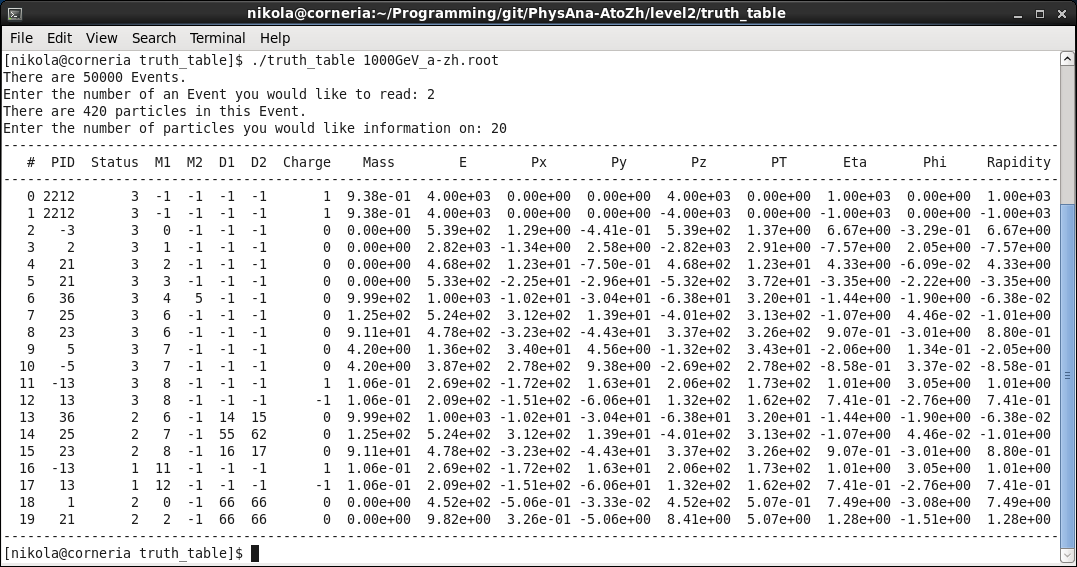
\includegraphics[width = \linewidth]{truth_table_screenshot.png}

\bigskip

Before analyzing Figure X, it is worth taking a look at the code for truth\_table in the main.cpp file in the truth\_table directory. With a basic understanding of ROOT and C++, this code should be straight forward. However, you may want to play around with which branches to read data from. For example, the code can be easily modified to read the Electron branch of our ROOT files instead of the Particle branch, and to output a table of information about the Electron objects in the Electron branch. To do this, for example, you could simply change the line

\begin{verbatim}
	TClonesArray * branchParticle = tr->UseBranch("Particle");
\end{verbatim}

to something like

\begin{verbatim}
	TClonesArray * branchElectron = tr->UseBranch("Electron");
\end{verbatim}

Then you could loop through the Electron objects in this branch and output their information using something like the following.

\begin{verbatim}
	for (int64_t i = 0; i < branchElectron->GetEntries(); i++)
	{
	        Electron * electron = (Electron*) branchElectron->At(i);

	        cout << electron->PT;

	        ...
	}
\end{verbatim}

Doing these small programming exercises will help to familiarize yourself with this type of analysis programming, and make reading and modifying future larger analysis programs easier. You are encouraged at any point throughout this tutorial to experiment with modifying the source code of the tutorial programs, and will indeed have to to carry out some of the analysis exercises presented here, or your own analysis.

\bigskip

Now, let's return to Figure X, and analyze each piece of the output truth particle information to understand the structure of a truth particle and of our Event.

\bigskip

The physical variables, such as Mass and E, should be evident. However, I should clarify the meaning of \#, PID, Status, M1, M2, D1, and D2.

\bigskip

\# simply refers to the index of a particle. The Particle branch in our ROOT files contain an array of GenParticle objects, each object corresponding to a truth particle. \# here refers to the index of a truth particle in that array. You can see in the code for truth\_table that we are outputting our truth particle information starting from the first index in the GenParticle array.

\bigskip

PID stands for "Particle ID." Each particle, such as electrons, anti muons, protons, etc, is identified here by an integer. For example, 13 refers to muons and 23 refers to Z bosons. A complete list of the PIDs for various particles is available at the following url.

\bigskip

\url{http://www.physics.ox.ac.uk/CDF/Mphys/old/notes/pythia_codeListing.html}

\bigskip

The Status of a particle can be either 3, 2, or 1. Status 3 refers to truth particles output from MadGraph, before parton showers are simulated by Pythia. Thus, for our AZH process, we would expect there to be exactly 2 Status 3 electrons or exactly 2 Status 3 muons. In the table output above, we can see that there are indeed exactly 2 Status 3 muons (2 Status 3 particles with PID 13). (You may be wondering if there are more Status 3 particles listed later in the table, as the table only lists the first 20 truth particles. You can verify for yourself with the program that all Status 3 particles occur at the beginning of the GenParticle array.) Status 2 particles are intermediate between Status 3 and Status 1 particles. Status 1 particles are final state particles - these are the truth particles left over at the end of the MadGraph and Pythia simulation processes (but before the Delphes detector response simulation, of course).

\bigskip

M1, M2, D1, and D2 refer to the indices of the mother and daughter particles of a particle. For example, we can see in Figure X that the index of the mother particle of particle \#12 (a muon) is particle \#8 (a Z boson). Using these variables, you can scan through a table to see the decay chains of all truth particles. You can do this either by eye, or by writing a program.

\subsubsection*{Exercises}

As an exercise at this point, you could write a program to count up all truth electrons in an Event, and use the M1 and M2 member variables to find the ultimate mother particle of these electrons. You can verify that the ultimate mother of all electrons is one of the Status 3 particles from the original MadGraph process.

\subsection{truth\_histogram}

The program truth\_histogram takes a ROOT file with a Particle branch as input, and outputs a histogram of the PT distribution of all Status 1 electrons (PID 11) and positrons (PID -11) in the Particle branch.

\bigskip

The code for truth\_histogram is located at the following url in the PhysAna-AtoZh git repository.

\bigskip

\url{https://github.com/schsu/PhysAna-AtoZh/tree/master/level2/truth_table}

\bigskip

To compile and run it, run

\begin{verbatim}
	make
\end{verbatim} 

in the truth\_histogram directory and then run

\begin{verbatim}
	./truth_histogram
\end{verbatim}

The program should output the following usage statement.

\begin{verbatim}
	usage: ./truth_histogram inputFile
\end{verbatim}

The program requires the user to provide the path to a ROOT file as commandline input. The program is not interactive - it just outputs the file "truth\_electron\_pt.eps" in present working directory. The output EPS file should look something like Figure Y.

\bigskip

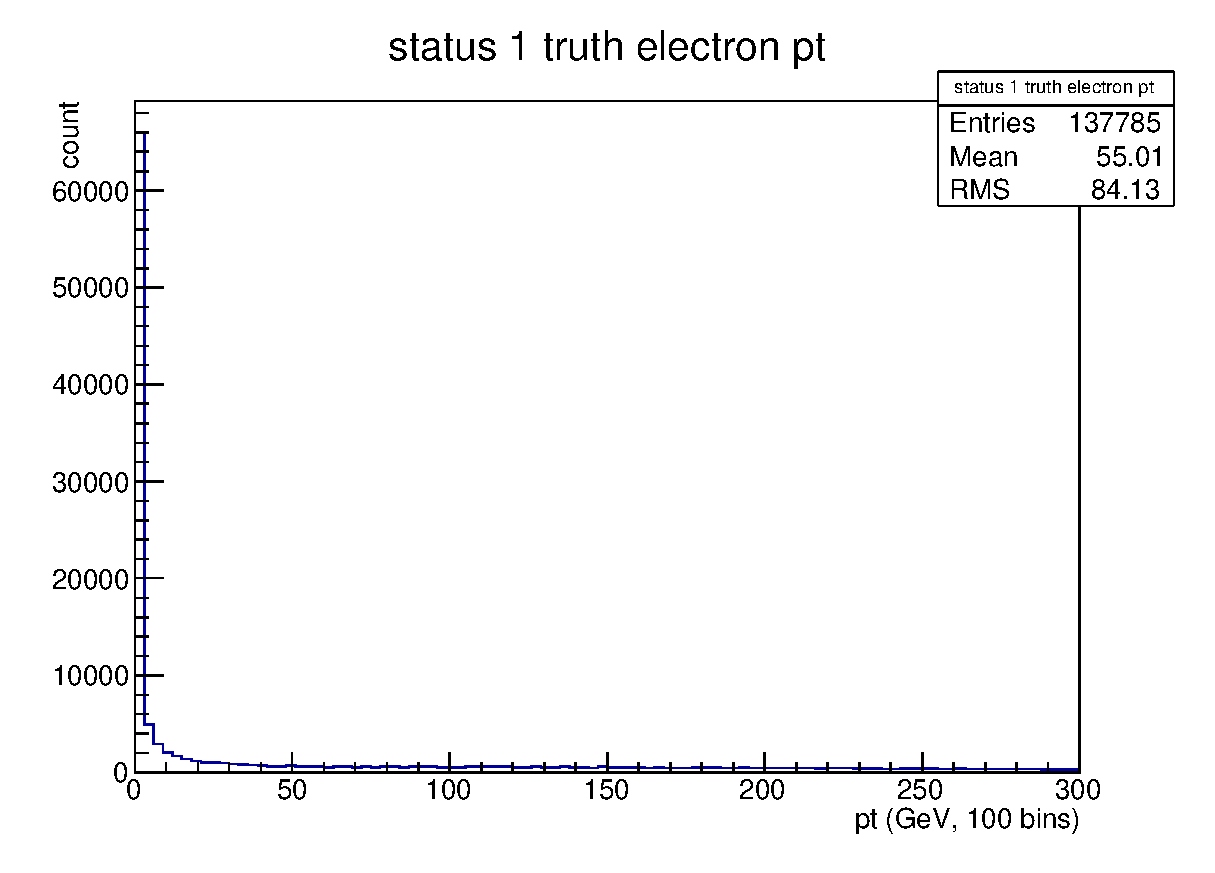
\includegraphics[width = \linewidth]{truth_electron_1_pt.eps}

\bigskip

Now we are ready to make some real physics analysis plots! The source code for truth\_histogram is very short, so it should be very easy to modify to output truth particle histograms of whatever you may be interested in - Status 1 electron PT, Status 3 muon energy, Status 3 Z boson Eta, you name it. For now, let's discuss the plot in Figure Y, and some real physics for a moment.

\bigskip

We see in Figure Y that the vast majority of Status 1 electrons have very low PT. However, the AZH process we are trying to analyze should produce 2 electrons (or muons) which decay from a Z boson. The Z boson has a mass of around 90 GeV, while an electrons only has a mass of 0.05 GeV, so the vast majority of the Z boson's mass should go into the electrons momentum. Thus, we should expect our electrons to have high PT. Why, then, do most of our Status 1 electrons have low PT? To answer that, let's first plot the PT distribution of Status 3 electrons. We know that Status 3 electrons are the electrons which decayed from our Z boson, whereas Status 1 electrons may have been produced by our parton shower. This plot is displayed in Figure Z.

\bigskip

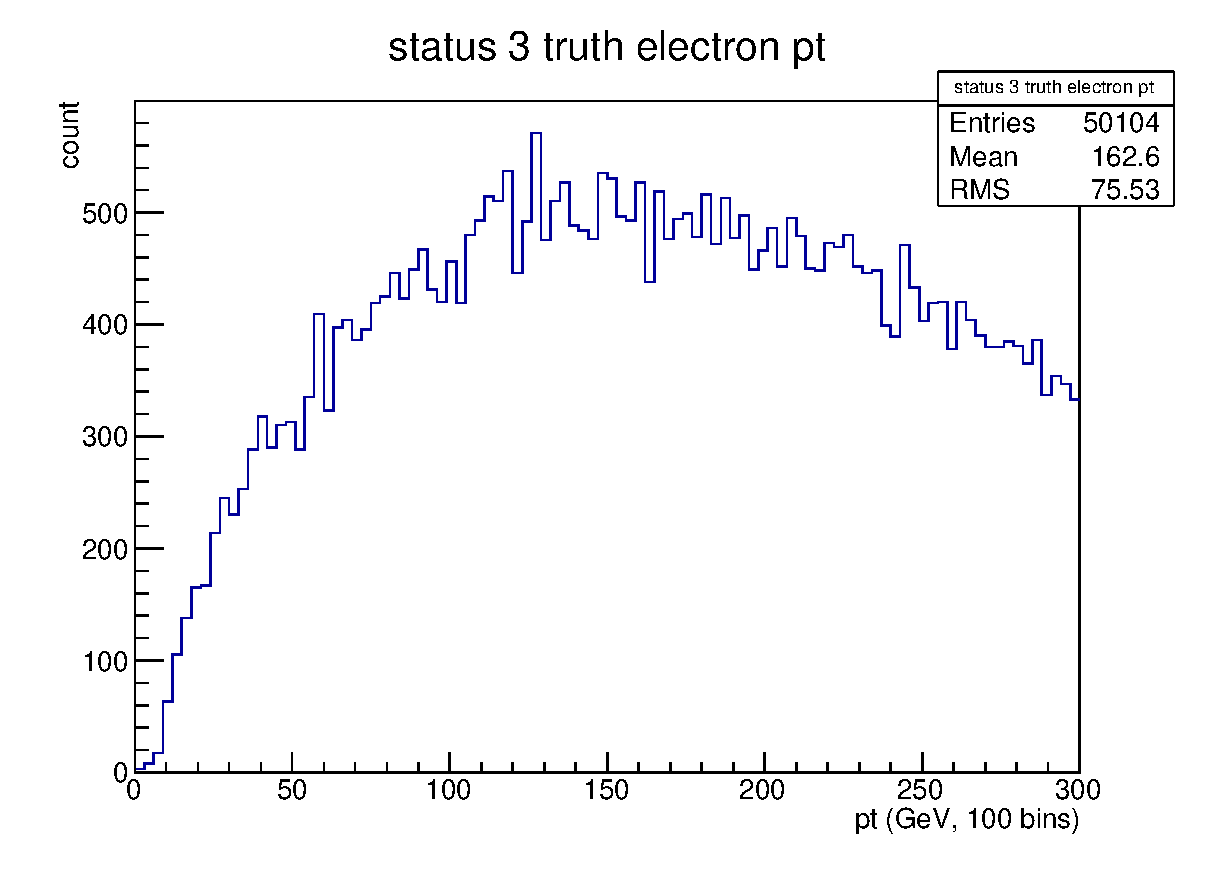
\includegraphics[width = \linewidth]{truth_electron_3_pt.eps}

\bigskip

Indeed, we see that Status 3 electrons have a high PT distribution! In fact, we see that there are much less Status 3 electrons in our Particle branch than Status 1 electrons. This should make sense after studying the truth\_table program and its output. Now we can ask ourselves, does it make sense that electrons produced by our parton showers have low PT? ...

\bigskip

Understanding these plots is at the heart of physics analysis. These PT distributions offer early motivation for a low PT cut, however, since we are studying truth particle information, and not detected particles (the step performed by Delphes), it is a bit too early to discuss cuts. This is left for Level 3 of this tutorial.

\subsubsection*{Exercises}

An example of real physics analysis was presented with comparing the PT distribution of Status 3 and Status 1 electrons. With very slight modifications to the truth\_histogram code, you could at this point study many kinematic aspects of our truth particles. For example, you could study the opening angle distribution of the 2 electrons (or muons) which decay from our Z boson, or maybe make a 2D histogram of this opening angle distribution vs combined PT of the 2 electrons (or muons). You could also verify that the mass of the combined electrons' 4vector is indeed the mass of our Z boson. You could similarly verify that the combined 4vector mass of the 2 bottom quarks which decayed from our Higgs is indeed the mass of our Higgs. You could study the opening angle distribution of our Higgs and our Z boson which decayed from A. Being able to produce these plots is critical in all following analysis, and you should feel free to both practice producing these plots, and thinking up good questions which could be answered by viewing these plots.

\section{Level 3: Detected Particle Study}

\end{document}
